\documentclass[11pt]{article}
\usepackage[a4paper,margin=1in]{geometry}
\usepackage{amsmath,amssymb,amsfonts,mathtools,bm}
\usepackage{tikz}
\usetikzlibrary{arrows.meta}

\pagestyle{empty}

\newcommand{\R}{\mathbb{R}}
\newcommand{\N}{\mathbb{N}}
\newcommand{\eps}{\varepsilon}
\newcommand{\one}{\mathbf{1}}
\newcommand{\softmax}{\operatorname{softmax}}
\newcommand{\TopK}{\operatorname{TopK}}
\newcommand{\row}{\operatorname{row}}
\newcommand{\norm}[1]{\left\lVert #1 \right\rVert}

\begin{document}


\section*{Resolution}

This architecture uses learned vectors, not hand-built feature functions.
The equations below keep three objects explicit:
\[
\text{direction},\qquad \text{magnitude},\qquad \text{routing}.
\]

The direction lives on the unit hypersphere:
\[
S^{d-1}=\{u\in\mathbb{R}^{d}:\|u\|_2=1\}.
\]

The magnitude is kept separately:
\[
 x_i \mapsto (\widehat{x}_i,m_i),
 \qquad
 \widehat{x}_i=\frac{x_i}{\|x_i\|_2+\varepsilon},
 \qquad
 m_i=\|x_i\|_2.
\]

The graph is not a feature system. The graph is a routing constraint:
\[
G\to M\to B\to P.
\]

\section*{Unit Hypersphere}

\[
S^1\subset\mathbb{R}^2,
\qquad
S^2\subset\mathbb{R}^3,
\qquad
S^{d-1}\subset\mathbb{R}^{d}.
\]

\begin{center}
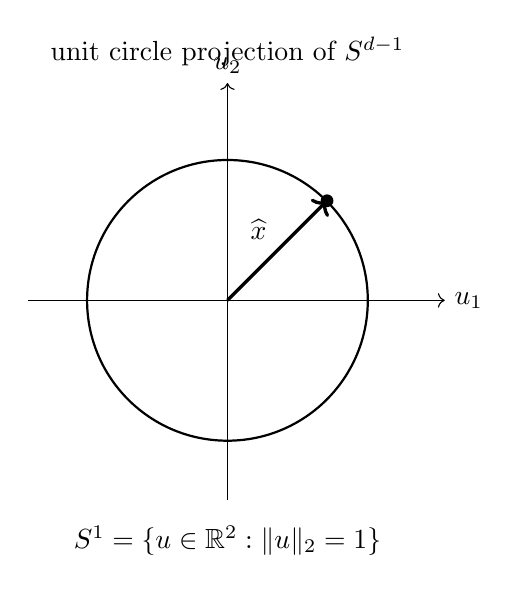
\begin{tikzpicture}[scale=1.15]
  \draw[->] (-2.2,0) -- (2.4,0) node[right] {$u_1$};
  \draw[->] (0,-2.2) -- (0,2.4) node[above] {$u_2$};
  \draw[thick] (0,0) circle (1.55);
  \draw[very thick,->] (0,0) -- (1.10,1.10) node[midway,above left] {$\widehat{x}$};
  \fill (1.10,1.10) circle (2pt);
  \node at (0,-2.65) {$S^1=\{u\in\mathbb{R}^2:\|u\|_2=1\}$};
  \node at (0,2.75) {unit circle projection of $S^{d-1}$};
\end{tikzpicture}
\end{center}

\[
\widehat{x}_i^{\mathsf T}\widehat{x}_j=\cos\theta_{ij}
\]

\[
\|\widehat{x}_i-\widehat{x}_j\|_2^2=2(1-\cos\theta_{ij})
\]


\section*{Projection Preservation}

The lower-dimensional representation is not identical to the higher-dimensional representation.
It is accepted only when the relevant geometry is approximately preserved.

\[
R\in\mathbb{R}^{k\times d},
\qquad
k<d
\]

\[
z_i=R\widehat{x}_i,
\qquad
\widehat{z}_i=\frac{z_i}{\|z_i\|_2+\varepsilon}
\]

\[
\widehat{x}_i\in S^{d-1},
\qquad
\widehat{z}_i\in S^{k-1}
\]

\[
(1-\delta)\|\widehat{x}_i-\widehat{x}_j\|_2^2
\leq
\|R\widehat{x}_i-R\widehat{x}_j\|_2^2
\leq
(1+\delta)\|\widehat{x}_i-\widehat{x}_j\|_2^2
\]

\[
\|\widehat{x}_i-\widehat{x}_j\|_2^2
=
2\left(1-\widehat{x}_i^{\mathsf T}\widehat{x}_j\right)
\]

\[
\|\widehat{z}_i-\widehat{z}_j\|_2^2
=
2\left(1-\widehat{z}_i^{\mathsf T}\widehat{z}_j\right)
\]

Therefore:

\[
\|\widehat{x}_i-\widehat{x}_j\|_2^2
\approx
\|\widehat{z}_i-\widehat{z}_j\|_2^2
\]

\[
\Longrightarrow
\qquad
\widehat{x}_i^{\mathsf T}\widehat{x}_j
\approx
\widehat{z}_i^{\mathsf T}\widehat{z}_j
\]

\[
\Longrightarrow
\qquad
\cos\theta_{ij}^{(d)}
\approx
\cos\theta_{ij}^{(k)}
\]

\[
\boxed{
S^{d-1}\xrightarrow{\ R\ }S^{k-1}
\qquad
\text{if distances and cosines are preserved within }\delta
}
\]

\[
\boxed{
\text{higher dimension}\to\text{lower dimension}
\neq
\text{same object}
}
\]

\[
\boxed{
\text{higher dimension}\to\text{lower dimension}
\approx
\text{same alignment geometry}
}
\]


\section*{Architecture}

\subsection*{Map}

\[
\mathcal{A}_{\Theta,G}:D \mapsto Y
\]

\[
D
\xrightarrow{\Theta_0}
X^{(0)}
\xrightarrow{\nu}
(\widehat X^{(0)},m^{(0)})
\xrightarrow{G}
M
\xrightarrow{\mathcal T_{\Theta}}
Y
\xrightarrow{\nu}
(\widehat Y,m^Y)
\]

\[
n,d,L,H,d_h,d_v,k\in\N,
\qquad
\eps>0
\]

\[
X^{(0)}=F_{\Theta_0}(D),
\qquad
X^{(\ell)}\in\R^{n\times d}
\]

\[
x_i^{(\ell)}=\row_i(X^{(\ell)})^{\mathsf T}\in\R^d,
\qquad
0\leq \ell \leq L
\]

\[
m_i^{(\ell)}
=
\norm{x_i^{(\ell)}}_2
=
\sqrt{(x_i^{(\ell)})^{\mathsf T}x_i^{(\ell)}}
\]

\[
\widehat x_i^{(\ell)}
=
\frac{x_i^{(\ell)}}{m_i^{(\ell)}+\eps},
\qquad
\widehat x_i^{(\ell)}\in S^{d-1}
\]

\[
S^{d-1}=\{u\in\R^d:\norm{u}_2=1\}
\]

\[
\widehat X^{(\ell)}
=
\begin{bmatrix}
(\widehat x_1^{(\ell)})^{\mathsf T}\\
(\widehat x_2^{(\ell)})^{\mathsf T}\\
\vdots\\
(\widehat x_n^{(\ell)})^{\mathsf T}
\end{bmatrix}
\in\R^{n\times d}
\]

\[
m^{(\ell)}
=
\begin{bmatrix}
m_1^{(\ell)}\\
m_2^{(\ell)}\\
\vdots\\
m_n^{(\ell)}
\end{bmatrix}
\in\R^{n\times 1}
\]

\[
r_i^{(\ell)}=\log(m_i^{(\ell)}+\eps),
\qquad
r^{(\ell)}
=
\begin{bmatrix}
r_1^{(\ell)}\\
r_2^{(\ell)}\\
\vdots\\
r_n^{(\ell)}
\end{bmatrix}
\]

\[
Z^{(\ell)}=
\begin{bmatrix}
\widehat X^{(\ell)} & r^{(\ell)}
\end{bmatrix}
\in\R^{n\times(d+1)}
\]

\subsection*{Graph Mask}

\[
G=(V_G,E_G),
\qquad
V_G=\{1,2,\ldots,n\},
\qquad
E_G\subseteq V_G\times V_G
\]

\[
M_{ij}=\mathbf{1}_{(i,j)\in E_G},
\qquad
M\in\{0,1\}^{n\times n}
\]

\[
M^+_{ij}=\max(M_{ij},\delta_{ij})
\]

\[
C_{ij}^{(\ell)}
=
(\widehat x_i^{(\ell)})^{\mathsf T}\widehat x_j^{(\ell)}
\]

\[
\Delta_{ij}^{(\ell)}
=
\norm{\widehat x_i^{(\ell)}-\widehat x_j^{(\ell)}}_2^2
=
2(1-C_{ij}^{(\ell)})
\]

\[
\mathcal K_i^{(\ell)}=\TopK_j(C_{ij}^{(\ell)},k)
\]

\[
T_{ij}^{(\ell)}=\mathbf{1}_{j\in \mathcal K_i^{(\ell)}}
\]

\[
\overline M_{ij}^{(\ell)}=M^+_{ij}T_{ij}^{(\ell)}
\]

\[
B_{ij}^{(\ell)}
=
\begin{cases}
0,&\overline M_{ij}^{(\ell)}=1\\
-\infty,&\overline M_{ij}^{(\ell)}=0
\end{cases}
\]

\subsection*{Sparse Attention}

\[
W_Q^{(\ell,h)},W_K^{(\ell,h)}\in\R^{d\times d_h},
\qquad
W_V^{(\ell,h)}\in\R^{(d+1)\times d_v}
\]

\[
W_O^{(\ell)}\in\R^{Hd_v\times d},
\qquad
W_R^{(\ell)}\in\R^{d\times d}
\]

\[
Q^{(\ell,h)}=\widehat X^{(\ell)}W_Q^{(\ell,h)}
\]

\[
K^{(\ell,h)}=\widehat X^{(\ell)}W_K^{(\ell,h)}
\]

\[
V^{(\ell,h)}=Z^{(\ell)}W_V^{(\ell,h)}
\]

\[
S^{(\ell,h)}
=
\frac{Q^{(\ell,h)}(K^{(\ell,h)})^{\mathsf T}}{\sqrt{d_h}}
+
B^{(\ell)}
\]

\[
P_{ij}^{(\ell,h)}
=
\frac{\exp(S_{ij}^{(\ell,h)})}
{\sum_{q=1}^{n}\exp(S_{iq}^{(\ell,h)})}
\]

\[
P^{(\ell,h)}=\softmax_j(S^{(\ell,h)})
\]

\[
P_{ij}^{(\ell,h)}=0
\qquad
\forall\;\overline M_{ij}^{(\ell)}=0
\]

\[
O^{(\ell,h)}=P^{(\ell,h)}V^{(\ell,h)}
\]

\[
O^{(\ell)}
=
\begin{bmatrix}
O^{(\ell,1)}&O^{(\ell,2)}&\cdots&O^{(\ell,H)}
\end{bmatrix}
W_O^{(\ell)}
\]

\[
R^{(\ell)}=X^{(\ell)}W_R^{(\ell)}+O^{(\ell)}
\]

\[
X^{(\ell+1)}=R^{(\ell)}
\]

\[
Y=X^{(L)}
\]

\[
y_i=\row_i(Y)^{\mathsf T},
\qquad
m_i^Y=\norm{y_i}_2,
\qquad
\widehat y_i=\frac{y_i}{m_i^Y+\eps}
\]

\[
\widehat Y
=
\begin{bmatrix}
\widehat y_1^{\mathsf T}\\
\widehat y_2^{\mathsf T}\\
\vdots\\
\widehat y_n^{\mathsf T}
\end{bmatrix},
\qquad
m^Y
=
\begin{bmatrix}
m_1^Y\\
m_2^Y\\
\vdots\\
m_n^Y
\end{bmatrix}
\]

\[
R^\star\in\R^{n\times d},
\qquad
r_i^\star=\row_i(R^\star)^{\mathsf T}
\]

\[
m_i^\star=\norm{r_i^\star}_2,
\qquad
\widehat r_i^\star=\frac{r_i^\star}{m_i^\star+\eps}
\]

\subsection*{Loss}

\[
\mathcal L_1
=
\sum_{i=1}^{n}
\left(1-\widehat y_i^{\mathsf T}\widehat r_i^\star\right)
\]

\[
\mathcal L_2
=
\sum_{i=1}^{n}
\left(\log(m_i^Y+\eps)-\log(m_i^\star+\eps)\right)^2
\]

\[
\mathcal L_3
=
\sum_{\ell=0}^{L-1}\sum_{h=1}^{H}
\norm{P^{(\ell,h)}\odot(\one\one^{\mathsf T}-\overline M^{(\ell)})}_F^2
\]

\[
\mathcal L_4
=
\sum_{\ell=0}^{L-1}
\norm{X^{(\ell+1)}-X^{(\ell)}}_F^2
\]

\[
\mathcal L_{\Theta}
=
\lambda_1\mathcal L_1+
\lambda_2\mathcal L_2+
\lambda_3\mathcal L_3+
\lambda_4\mathcal L_4
\]

\subsection*{Update}

\[
\Theta_{t+1}=\Theta_t-\eta \nabla_{\Theta}\mathcal L_{\Theta}
\]

\[
X_{t+1}^{(0)}=Y_t
\]

\[
D
\to
X
\to
(\widehat X,m)
\to
G
\to
M
\to
(Q,K,V)
\to
P
\to
Y
\to
(\widehat Y,m^Y)
\]

\[
\boxed{
\mathcal A_{\Theta,G}
=
\nu\circ \mathcal T_{\Theta}\circ M_G\circ \nu\circ F_{\Theta_0}
}
\]

\end{document}
